\documentclass[12pt]{article}
\usepackage[utf8]{inputenc}
\usepackage{float}
\usepackage{amsmath}
\usepackage{graphicx}


\usepackage[hmargin=3cm,vmargin=6.0cm]{geometry}
%\topmargin=0cm
\topmargin=-2cm
\addtolength{\textheight}{6.5cm}
\addtolength{\textwidth}{2.0cm}
%\setlength{\leftmargin}{-5cm}
\setlength{\oddsidemargin}{0.0cm}
\setlength{\evensidemargin}{0.0cm}

%misc libraries goes here
%\usepackage{fitch}


\begin{document}

\section*{Student Information } 
%Write your full name and id number between the colon and newline
%Put one empty space character after colon and before newline
Full Name :  Can Erdoğar \\
Id Number :  1942069 \\

% Write your answers below the section tags
\section*{Answer 1}
a) Telephone numbers : Nominal \\
b) Ratings of fiction books-excellent, good, fair, poor : Ordinal \\
c) Amounts of money spent on a medical checkup : Ratio \\
d) Scores on a data mining exam : Interval \\
e) Blood Types : Nominal \\
f) The ages of METU students : Ratio \\
g) The movie ratings : Ordinal \\
h) Colors of METU t-shirts in ODTUDEN Shop : Nominal\\
i) Temperatures of hot tubs in local health clubs : Interval \\

\section*{Answer 2}
To make the probability of each item being selected equal.\\

\section*{Answer 3}
workout time is independent \\
the risk of catching a cold is dependent \\
meditation is independent \\
making rational decisions is dependent \\
\section*{Answer 4}
\begin{figure}[H]
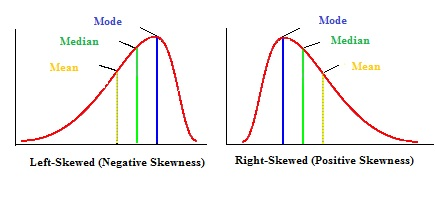
\includegraphics[width=8cm]{pearson-mode-skewness.jpg}
\centering
\end{figure}

\begin{figure}[H]
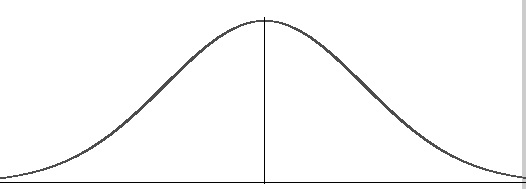
\includegraphics[width=8cm]{normal-distribution-probability.jpg}
\centering
\end{figure}


\section*{Answer 5}
a-mode \\
b-median \\
c-mode \\
d-mean \\
e-mean \\
f-median \\

\section*{Answer 6}
Then, there is no mode.\\

\section*{Answer 7}

Mean is 27.2, Median is 19, Mode is 17, midrange is 38 \\

\section*{Answer 8}

variance is 13.1, sample standard deviation is 3.61939221417 \\

\section*{Answer 9}

range is 306, variance is 6638.55555556, standard deviation is 81.4773315442 \\

\section*{Answer 10}

No, actually if two events are mutually exclusive it is only in a special case that they can be independent. The definitions state that two events A,B are\\
mutually exclusive iff $P(A \cap B) = 0$, i.e. $A \cap B = \emptyset$ \\
independent iff $P(A \cap B) = P(A)P(B)$ \\
Assume know that A,B are both mutually exclusive and independent. Then combining the above yields \\
$P(A)P(B)=0$\\
which implies that at least one of the $P(A)$ and $P(B)$ has to be zero.\\

\section*{Answer 11}

Normal distributions are symmetric, unimodal, and asymptotic, and the mean, median, and mode are all equal.\\

A normal distribution is perfectly symmetrical around its center. That is, the right side of the center is a mirror image of the left side. There is also only one mode, or peak, in a normal distribution. Normal distributions are continuous and have tails that are asymptotic, which means that they approach but never touch the x-axis. The center of a normal distribution is located at its peak, and 50\% of the data lies above the mean, while 50\% lies below. It follows that the mean, median, and mode are all equal in a normal distribution. \\

\section*{Answer 12}

Mean and deviation affects the shape and the position of a normal distribution curve \\

Formula is $\frac{1}{\sigma \sqrt{2 \pi}} e^{- \frac{1}{2} {(\frac{x-u}{\sigma})}^2}$

\section*{Answer 13}

A standard normal distribution is a normal distribution with mean 0 and standard deviation 1. The total area under the normal curve is equal to 1.\\

\section*{Answer 14}
A z-test is a statistical test used to determine whether two population means are different when the variances are known and the sample size is large. \\
A t-test is an analysis of two populations means. A t-test with two samples is commonly used with small sample sizes, testing the difference between the samples when the variances of two normal distributions are not known. \\
There are two types of chi-square test. A chi-square goodness of fit test determines if a sample data matches a population.A chi-square test for independence compares two variables in a contingency table to see if they are related. In a more general sense, it tests to see whether distributions of categorical variables differ from each another.\\
\section*{Answer 15}
Chi-square \\
\section*{Answer 16}

What is meant by positive relationship between two variables is that when one variable decreases as the other variable decreases, or one variable increases while the other increases. Two variables move in tandem. \\

What is meant by positive relationship between two variables is that when one variable increases then the other decreases, and vice versa. \\

\section*{Answer 17}
Assume that we have a collection of paired data containing the sample point $(x , y)$, that $\hat y$ is the predicted value of y, and that the mean of the sample y-values is $\bar y$ \\
The total variation about a regression line is the sum of the squares of the differences between the y-value of each ordered pair and the mean of y. \\
total variation = $\sum {(y - \bar{y})}^2 $ \\
The explained variation is the sum of the squared of the differences between each predicted y-value and the mean of y. \\
explained variation = $\sum {(\hat{y} - \bar{y})}^2 $ \\
The unexplained variation is the sum of the squared of the differences between the y-value of each ordered pair and each corresponding predicted y-value. \\
unexplained variation = $\sum {(y - \hat{y})}^2 $ \\

\section*{Answer 18}

The correlation coefficient is a measure that determines the degree to which two variables' movements are associated. \\
the value of the linear correlation coefficient will be zero if there is no relationship between the variables.

\end{document}

​

